\documentclass[a4paper,11pt, twocolumn]{article}
\usepackage[margin=0.8in]{geometry}
\usepackage{xcolor}
\usepackage{graphicx} %package to manage images
\graphicspath{ {./images/} }
\usepackage{float}

\title{PIC Microcontroller}
\author{Revision sheet}
\date{}

\usepackage{fancyhdr}
\pagestyle{fancy}
\fancyhead{} % clear all header fields
\renewcommand{\headrulewidth}{0pt} % no line in header area
\fancyfoot{} % clear all footer fields
\renewcommand{\footrulewidth}{0.4pt}
\fancyfoot[C]{\thepage} % page number in centre of the page
\fancyfoot[R]{\footnotesize Thomas Boxall \\ } % right hand footer has author name on top line and images reference on bottom line
\fancyfoot[L]{\footnotesize PIC Microcontroller \\ Revision sheet} % left hand footer has title of document on top line and 'Revision Sheet' on bottom line


\begin{document}

\maketitle
\thispagestyle{fancy}

% CONTENTS OF THE REVISION SHEET HERE
\section{Flowcharts}
Flowcharts are a graphical way of representing flow through a program. Flowcharts are built from symbols, with each symbol having a different meaning. The symbols are outlined below.
\begin{figure}[H]
    \centering
    
\includegraphics[width=\linewidth]{fcTerminator.jpg}
    \caption{Terminator block}
\end{figure}
\noindent The terminator block indicates the start or the end of a program.
\begin{figure}[H]
    \centering
    
\includegraphics[width=\linewidth]{fcProcess.jpg}
    \caption{Process block}
\end{figure}
\noindent The process block indicates a calculation or delay.
\begin{figure}[H]
    \centering
    
\includegraphics[width=\linewidth]{fcDecision.jpg}
    \caption{Decision block}
\end{figure}
\noindent The decision block tests a condition with a \verb|yes| or \verb|no| answer. The program will follow a different route depending on the answer.
\begin{figure}[H]
    \centering
    
\includegraphics[width=\linewidth]{fcIO.jpg}
    \caption{Input/Output block}
\end{figure}
\noindent The input/Output block indicates data being read into or written from the program.
\begin{figure}[H]
    \centering
    
\includegraphics[width=\linewidth]{fcSubroutine.jpg}
    \caption{Subroutine block}
\end{figure}
\noindent The subroutine block indicates the program should run another sub-program then return to where it was called from (the location of the subroutine block).

\section{Parts Of The PIC Microcontroller}
The PIC Microcontroller has a number of parts which are useful.
\subsection{Pinout}
The pinout of the PIC Microcontroller can be seen below.
\begin{figure}[H]
    \centering
    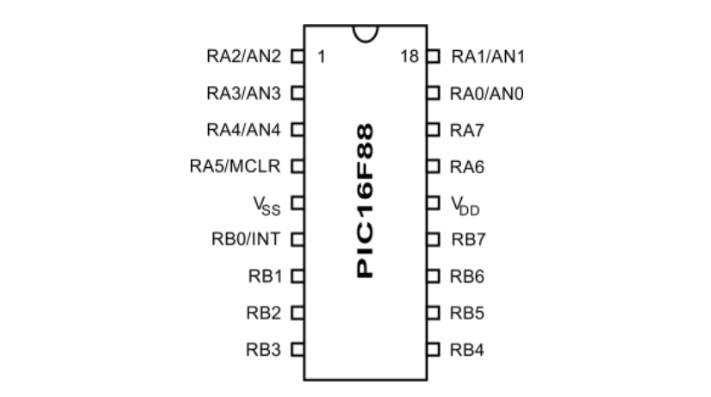
\includegraphics[width=\linewidth]{pinout.jpg}
    \caption{Pinout of the PIC16F88}
\end{figure}
\subsection{Registers}
A register is an 8-bit memory storage location. Each bit of the register is independantly controllable/ accessible. There are a number of different registers which are important.
\subsubsection{The Working (W) Register}
The working (W) register is the only register into which data can be entered from the program. This means that data which is to be placed into another register or data which has come from another register which the CPU needs to access for processing, has to go via the W register. 
\subsubsection{The Data Direction Registers}
Each port has a data direction register. The contents of these registers sets the direction of the port bits. This generally only needs to happen once, at the beginning of the program. When setting the directions, 1 means input and 0 means output. The direction register for PORTA is called TRISA and the direction register for PORTB is called TRISB. 
\subsubsection{PORTA and PORTB registers}
The PORTA and PORTB registers hold the actual data that is present on the two ports. If the port bits are set as outputs, the contents of the W register can be copied to the port registers - changing the outputs. 
\subsubsection{STATUS register}
The STATUS register is used by the microcontroller for various functions. It's layout is shown on the formula booklet. The C bit (bit 0) will go logic high if an arithmetic operation resulted in a carry. The Z bit (bit 2) will go logic high if an arithmetic operation has resulted in zero. 

\section{Interrupts}
\subsection{Why Use Interrupts?}
Interrupts are used as they are more efficient. The alternative to using interrupts, is to use polling which is where an input is continually checked to see what it is and reacting then. Interrupts work by reacting as soon as something changes. Once the interrupt has been dealt with, the microcontroller returns to whatever it was doing before.
\subsection{Interrupt Service Routine}
The steps below outline the ISR.
\begin{enumerate}
    \item Save the contents of the W register to a variable (this is so that it can be re-filled after the ISR)
    \item Check if teh right interrupt happened by checking the external interrupt flag
    \item Execute the interrupt's code
    \item Clear the External Interrupt Flag, so that another interrupt can be triggered
    \item Restore the contents of the W register (copy the variable back into the W register)
    \item Return from the ISR.
\end{enumerate}
\subsubsection{Example ISR}
Shown below is an example ISR
\begin{verbatim}
    interrupt

        movwf w_save 
        ; copy w to save variable
        
        btfss INTCON, INT0IF
        ; check correct interrupt happened
        
        retfie
        ; if not, return to where was
        
        ; interrupt code here
        
        bcf INTCON, INT0IF
        ;clear interrupt flag
        
        movf w_save, W
        ;restore working register
        
        retfie
        ;return and re-set GIE bit

\end{verbatim}
\subsection{Defining The Interrupt}
The PIC has to be told where to find the ISR. The interrupt vector address is 04, this means that when an interrupt is triggered whatever the code at memory location 04 is will be run. The code below shows the declaration of this.
\begin{verbatim}
 ORG
    h'04'
    goto interrupt
\end{verbatim}
The code above should go near the start vector.

\section{PIC Microcontroller Assembly Language}
\subsection{List Of Commands}
\textit{This list is also available in the Data Booklet}
\begin{figure}[H]
    \centering
    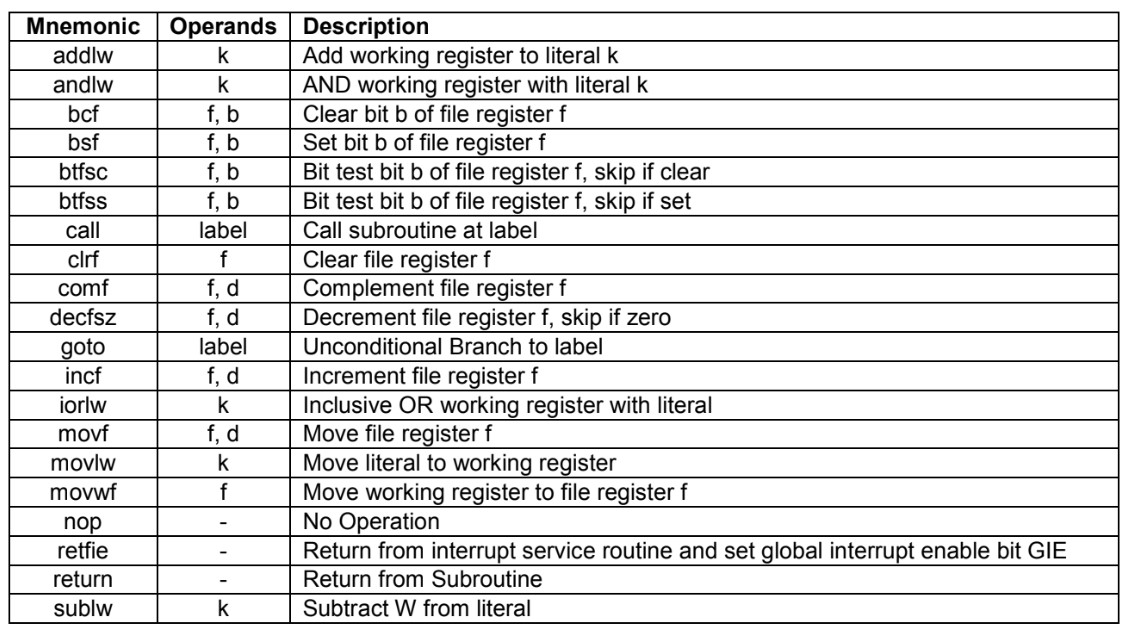
\includegraphics[width=\linewidth]{commands.jpg}
    \caption{Assembly language commands for the PIC Microcontroller}
\end{figure}
\subsection{Subroutines}
The example below shows a subroutine which flashes a LED for a short amount of time. We will assume that the LED is connected to bit 0 of PORTA.
\begin{verbatim}
    flash bsf PORTA, 0
            call wait100ms
            call wait100ms
            call wait100ms
            call wait100ms
            call wait100ms
            bcf PORTA, 0
            return
\end{verbatim}
The name of the subroutine is used at the top and then at the end the \verb|return| keyword is used. 
\subsection{Setting port Directions}
Example code to set the port direction is shown below. The code below will set all bits of PORTA to be input bits and all bits of PORTB to be output bits.
\begin{verbatim}
    movlw b'11111111'
    movwf TRISA
    movlw b'00000000'
    movwf TRISB
\end{verbatim}




\end{document}
